\documentclass[twoside]{article}

\usepackage[sc]{mathpazo} 
\usepackage[spanish, es-tabla]{babel}
\decimalpoint
\usepackage[utf8]{inputenc}

\usepackage[hmarginratio=1:1,top=32mm,columnsep=20pt]{geometry} % Document margins
\usepackage{multicol} % Used for the two-column layout of the document
\usepackage[hang, small,labelfont=bf,up,textfont=it,up]{caption} % Custom captions under/above floats in tables or figures
\usepackage{mathtools}
\usepackage{float} % Required for tables and figures in the multi-column environment - [H] needed
\usepackage{hyperref} % For hyperlinks in the PDF with labels

\usepackage{abstract} % Allows abstract customization
\renewcommand{\abstractnamefont}{\normalfont\bfseries} % Set the "Abstract" text to bold
\renewcommand{\abstracttextfont}{\normalfont\small\itshape} % Set the abstract itself to small italic text

\usepackage{titlesec} % Allows customization of titles

\titleformat{\section}[block]{\large\scshape\centering}{\thesection.}{1em}{} % Change the look of the section titles
\titleformat{\subsection}[block]{\large\centering}{\thesubsection.}{1em}{} % Change the look of the section titles

\usepackage{fancyhdr} % Headers and footers
\pagestyle{fancy} % All pages have headers and footers
\fancyhead{} % Blank out the default header
\fancyfoot{} % Blank out the default footer
\fancyhead[C]{Simulacion de Señal% based on TRACS 
\hspace{4pt} $\bullet$ \hspace{4pt} Enero 2019 } % Custom header text
\fancyfoot[RO,LE]{\thepage} % Custom footer text

%----------------------------------------------------------------------------
%	   TITLE SECTION
%----------------------------------------------------------------------------

\title{
	\vspace{-15mm}
	\fontsize{28pt}{10pt}
	\selectfont\textbf{Simulación de la Función de Autocorrelación de una señal}% Article title
}

\author{
	\large
	\textsc{Jaime D\'iez Gonz\'alez-Pardo}\\[4mm]
	\fontsize{28pt}{10pt} Universidad de Cantabria \\ % Your institution
	%\thanks{A thank you or further information}\\[2mm] % Your name
	\normalsize Fotónica \\ 
	%\normalsize{Compañeros:} \textsc{NOMBRE COMPANEROS }\\%\normalsize \href{mailto:john@smith.com}{john@smith.com} % Your email address
	%\vspace{5mm}
}

\date{ \today }


%----------------------------------------------------------------------------
%      · DOCUMENT
%----------------------------------------------------------------------------

\begin{document}


	\maketitle % Insert title


	\thispagestyle{fancy} % All pages have headers and footers

%----------------------------------------------------------------------------
%	  ABSTRACT
%----------------------------------------------------------------------------

	\begin{abstract}

		\noindent% Dummy abstract text

			Se ha obtenido la función de autocorrelación de una señal cosenoidal $I(t)$ de manera tanto analítica como numérica. Para el primer caso se ha resuelto la expresión obteniendo el valor de la integral. Para el caso de la resolución numérica se ha simulado dicha función para dos flujos distinto $\bar{I} = \{ 100, 10000 \}$, utilizando para ello la distribución Poissoniana. Ambos casos han sido calculados para tres amplitudes diferentes de $M = {0.1, 0.5, 1}$ obteniendo tanto para la resolución analitica como para la numérica, resultados similares.

	\end{abstract}

%----------------------------------------------------------------------------
%	  ARTICLE CONTENTS
%----------------------------------------------------------------------------

	\begin{multicols}{2} % Two-column layout throughout the main article text

		\section{Introducción} % Scope of the project = rad effects + minimization
							 
			La función de autocorrelación es una herramienta estadística que permite obtener patrones repetitivos dentro de una señal con un cierto ruido. Uno de sus usos más comunes en el procesamiento de señales, pues permite obtener diferentes parámetros tales como frecuencia o amplitud. La expresión de la función de autocorrelación se encuntra en la ecuación \ref{eq:autReal}

				\begin{equation}
					g^{(2)}(\tau) = \frac{\left< I(t)I(t+\tau)\right>}{\left< I(t)\right>^2}
					\label{eq:autReal}
				\end{equation}

			En la ecuación \ref{eq:autReal} aparecen la señal de entrada $I(t)$ y $\tau = kT$. Los valores utilizados han sido de $T = 0.001$ s y $k = {1, ..100}$. La expresión de la señal de entrada utilizada ha sido la que se muestra a continuación.

				\begin{equation}
					I(t) = \bar{I}[1+M\cos(\omega t)]
					\label{eq:Valors}
				\end{equation}

			En la ecuación \ref{eq:Valors} a parecen el flujo de fotones, $\bar{I}$ o intensidad media, la frecuencia angular $\omega$ y la amplitud $M$. A continuación se muestran los valores utilizados.

				\begin{equation}
					\begin{matrix}
					M = \{0.1, 0.5, 1\} \\ \\
					\bar{I} = \{100, 10000\} \\ \\
					\omega = \frac{2\pi}{P} = \frac{2\pi}{0.1}
					\end{matrix}
				\end{equation}

			Para obtener el valor promedio de la señal $\left<I\right>$ en el periodo se puede utilizar la integral.

				\begin{equation}
					\left<I\right> = \frac{1}{P} \int^{P}_0 I(t) dt					
					\label{eq:integ}
				\end{equation}

			Por otro lado, si tenemos en cuenta que el número de fotos en cada instante viene dado por una distribución poissoniana, se puede expresar la función de autocorrelación de la siguiente forma:

				\begin{equation}
					g^{(2)}(\tau) = \frac{\left< n(t)n(t+\tau)\right>}{\left< n(t)\right>^2}
					\label{eq:autPoiss}
				\end{equation}

			Donde $n(t)$ viene dado por la distribución de Poisson.

%\newpage
		\section{Resolución Analítica}

			En esta parte se trata de resolver la ecuación \ref{eq:autReal} a partir de obtener los valores de la integral \ref{eq:integ}. Para ello realizaremos las integrales del numerador y del denominador por separado. Puesto que se trata de una señal cosenoidal, parece obvio concluir que el promedio de $I$ será igual al valor medio ($\left< I(t)\right> = \bar{I}$), por lo que solo habra que resolver $\left< I(t)I(t+\tau)\right>$:

				\begin{equation}
				\begin{matrix}
					\left< I(t)I(t+\tau)\right> = \frac{1}{P} \int^{P}_0 I(t)I(t+\tau) dt \\ \\
					\left< I(t)I(t+\tau)\right> =  \bar{I}^2 \left[1 + \frac{M^2}{2}\cos(\omega\tau)\right]
				\end{matrix}
				\label{eq:AnaliticaInteg}
				\end{equation}

				\begin{equation}
					g^{(2)}(\tau) = 1 + \frac{M^2}{2}\cos(\omega\tau)
					\label{eq:Analitica}
				\end{equation}

			La resolución matemática de la ecuación \ref{eq:AnaliticaInteg} y la obtención de la ecuación \ref{eq:Analitica} se realiza en el apéndice \ref{appen:1}. Se representa la ecuación \ref{eq:Analitica} con los valores de $\omega$, $\tau$ y $M$ en la Figura \ref{Img:Anal}

				\begin{figure}[H]
					\centering
					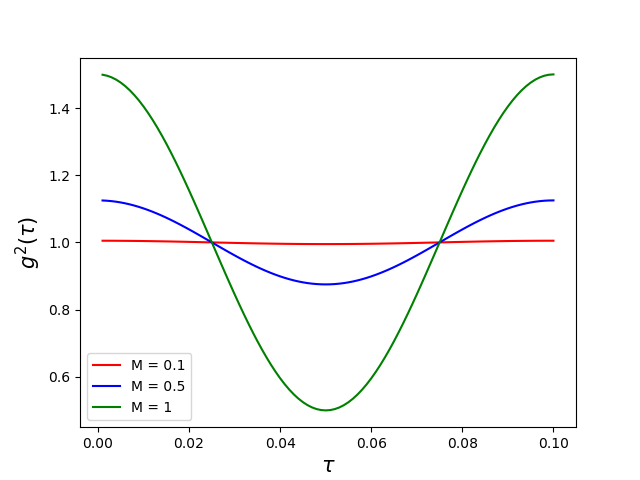
\includegraphics[scale=0.45]{../TheoInt.png}
					\caption{\label{Img:Anal}Solución Analitica de la función de autocorrelación $g^{(2)}(\tau)$ para tres valores distintos de $M = {0.1, 0.5, 1}$.}
				\end{figure}

		\section{Resolución Numérica}

			Para la resolución numérica se ha realizado una simulación mediante un código escrito en Python \cite{Resonador}. 

			Para ello, se ha obtenido el número de fotones $\bar{n}$ en intervalos de tiempo $(t,t+T)$

				\begin{equation}
					\bar{n}(t) = T*I(t+T-2)
					\label{eq:poiss}
				\end{equation}
			. Dicho valor se le ha pasado a una función llamada \textit{random.poisson()} de la librería \textit{numpy}. Esta función devuelve el valor de $n(t)$, por lo que una vez obtenidos dichos valores para todo $t$, se ha obtenido su media. De igual manera se ha hecho para $n(t+\tau)$ para cada uno de los $\tau$.

			Esta simulación se ha realizado $N = 100000$, es decir, con $N$ valores de $t$. A su vez, se ha realizado para cada uno de los $M$ y cada uno de los $\bar{I}$.

			En la Figura \ref{Img:10000} se muestran las funciones de autocorrelación obtenidas de forma numérica para un flujo de $\bar{I} = 10000$ y para tres amplitudes diferentes $M$.

				\begin{figure}[H]
					\centering
					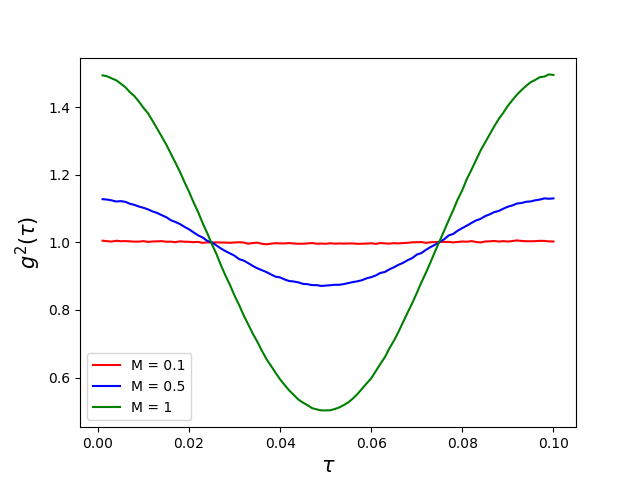
\includegraphics[scale=0.38]{../Int10000.png}
					\caption{\label{Img:10000}Solución numérica de la función de autocorrelación $g^{(2)}(\tau)$ para tres valores distintos de $M = {0.1, 0.5, 1}$ y flujo $\bar{I} = 10000$.}
				\end{figure}

			En la Figura \ref{Img:100} se muestran las funciones de autocorrelación obtenidas de forma numérica para un flujo de $\bar{I} = 100$ y para tres amplitudes diferentes $M$.

				\begin{figure}[H]
					\centering
					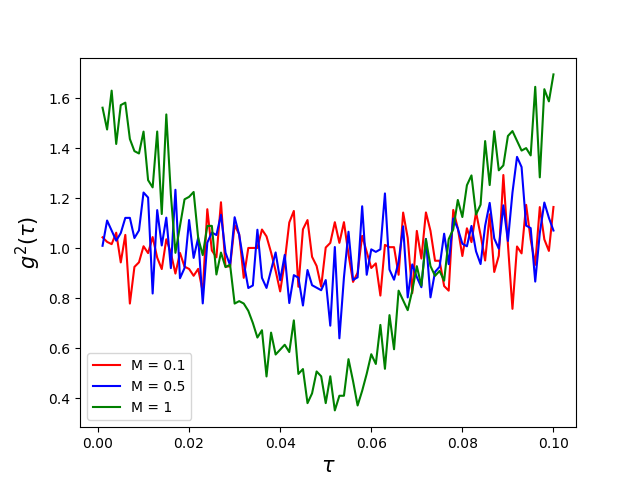
\includegraphics[scale=0.38]{../Int100.png}
					\caption{\label{Img:100}Solución numérica de la función de autocorrelación $g^{(2)}(\tau)$ para tres valores distintos de $M = {0.1, 0.5, 1}$ y flujo $\bar{I} = 100$.}
				\end{figure}

		\section{Conclusión}

			Se ha obtenido la función de correlación de una señal cosenoidal de manera tanto analítica com de manera numérica. En el caso de la resolución numérica se ha realizado para dos flujos de fotones distintos. Para el caso de un flujo de fotones de $\bar{I} = 10000$ se ha podido obtener unas funciones de autocorrelación muy similares a las obtenidas por el método analítico, observando poca discrepancia entre las Figuras \ref{Img:Anal} y \ref{Img:10000}. Sin embargo, en el caso de flujo $\bar{I} = 100$ se ha obtenido una función de autocorrelación con un enorme ruido, no puediendo compararla con la obtenida por el método analitico. No obtante, cabe destacar que, así como para amplitudes menores de $M= 0.1, 0.5$ la señal no se puede diferenciar del ruido, para el caso de $M=1$, pese a seguir teniendo un enorme ruido sí que es posible obtener la forma de la señal.

			De esta forma se aprecia como a medida que nuestra señal se debilita, y disminuye el número de fotones, el ruido aumenta, y como para la función de autocorrelación, el ruido obtenido es inversamente proporcional a la amplitud de la señal recibida.

	\end{multicols}

%----------------------------------------------------------------------------
%     APPENDIX
%----------------------------------------------------------------------------

\newpage

	    \appendix

	    	\section{Obtención de la Ecuación \ref{eq:AnaliticaInteg}}
	    		\label{appen:1}

	    		A continuación se muestra el desarrollo matemático realizado para la obtención de la integral:

	    		 \[\left< I(t)I(t+\tau)\right> = \frac{1}{P} \int^{P}_0 I(t)I(t+\tau) dt\]
	    		

	    		\[
		    			\left< I(t)I(t+\tau)\right> = \frac{1}{P} \int^{P}_0 I(t)I(t+\tau) dt = \frac {1}{0.1} \int^{0.1}_0 \bar{I}[1+M\cos(\omega t)]\bar{I}[1+M\cos(\omega t + \omega\tau)] \mathrm{d}t =
		    	\]

		    	\[
		    			= 10 \bar{I} \int^{0.1}_0 \{1 + M\cos(\omega t) + M \cos[\omega(t + \tau)] + M^2 \cos(\omega t) \cos[\omega(t+\tau)] \} \mathrm{d}t = 
	    		\]

	    		\[
	    			= \left\{\begin{matrix}
	    				\int^{0.1}_0 \mathrm{d}t = 0.1\\
	    				\int^{0.1}_0 M\cos(\omega t)\mathrm{d}t = \left[\frac{M}{\omega}\sin(\omega t)\right]^{0.1}_0 = 0\\ \\
	    				\int^{0.1}_0 M \cos[\omega(t + \tau)]\mathrm{d}t = \left[\frac{M}{\omega}\sin(\omega (t+\tau))\right]^{0.1}_0 = 0 \\ \\
	    			\end{matrix}\right\}
	    			= 10\bar{I} \left\{0.1 + \int^{0.1}_0 M^2 \cos(\omega t) \cos[\omega(t+\tau)] \right\} \mathrm{d}t
	    		\]

	    		\[
	    			\boxed{\cos(\omega t) \cos[\omega (t + \tau)] = \frac{1}{2}\{ \cos[\omega(2t + \tau)] + \cos(\omega \tau)\}}
	    		\]

	    		\[
	    			10\bar{I} \left\{0.1 + \int^{0.1}_0 M^2 \frac{1}{2}\{ \cos[\omega(2t + \tau)] + \cos(\omega \tau)\} \right\} \mathrm{d}t \rightarrow \left\{\begin{matrix}
	    				\int^{0.1}_0 \cos[\omega(2t + \tau)] + \cos(\omega \tau) \mathrm{d}t = \\ \\

	    				= \frac{M^2}{2}\left[\frac{1}{40\pi} \sin[20\pi (2t + \tau)] \right]_{0}^{0.1} + \left[t  \cos(\omega \tau) \right]_{0}^{0.1} = \\ \\

	    				 = \frac{M^2}{2}0.1\cos(\omega\tau)
	    			\end{matrix}\right\}
	    		\]

	    		\[
	    			\left< I(t)I(t+\tau)\right> = \bar{I}^2 \left[1+\frac{M^2}{2}\cos(\omega\tau)\right] \Rightarrow \boxed{g^{(2)}(\tau) = 1 + \frac{M^2}{2}\cos(\omega\tau)}
	    		\]
%----------------------------------------------------------------------------
%     BIBLIOGRAPHY
%----------------------------------------------------------------------------

	\bibliographystyle{unsrt}
	\bibliography{biblio}

\end{document}


%----------------------------------------------------------------------------
%            TEMPLATES
%----------------------------------------------------------------------------

%----------------------------------------------------------------------------
%            how to insert an image
%----------------------------------------------------------------------------

%	\begin{figure}[H]
%		\centering
%		\includegraphics[scale= ]{nombre de la imagen.jpg}
%		\caption{\label{Img:widgets}el pie de pagina que le quieras 	poner a la imagen}
%	\end{figure}
 
%----------------------------------------------------------------------------
%            how to insert a table
%----------------------------------------------------------------------------

%	\begin{table}[H]
%		\centering
%		\begin{tabular}{|c|c|c|c|}
%			\hline
%			\centering
%				Altura(h) & Distancia (d) & Elaboracion (e) & Longitud (l) \\
%				($\pm0.5$ mm) & ($\pm0.5$ mm) & ($\pm0.5$ mm) & ($\pm0.5$ mm) \\ \hline
%				 &  &  &  \\ \hline
%				 &  &  &  \\ \hline
%				 &  &  &  \\ \hline
%				 &  &  &  \\ \hline
%				 &  &  &  \\ \hline
%		         &  &  &  \\ \hline
%		\end{tabular}
%		\caption{\label{Tab:widgets}pie de pagina que le quieras poner}
%	\end{table}

%----------------------------------------------------------------------------
%             How to remove the label in equactions
%----------------------------------------------------------------------------

%	\begin{equation*}
%		
%	\end{equation*}

%----------------------------------------------------------------------------
%              How to set bibliography
%----------------------------------------------------------------------------

%\bibliographystyle{unsrt}
%\bibliography{biblio}
%
%Then you have to set a .bib document such as the next template
%
%	@book{nickname,
%	author = {},
%	title = {},
%	edition = {},
%	year = {},
%	volume = {},
%	ISBN = {}
%	}
%
%	@ARTICLE{nickname,
%	author = {},
%	title = {},
%	year = {},
%	volume = {},
%	}


%----------------------------------------------------------------------------
%              END
%----------------------------------------------------------------------------
